\chapter{State-of-the-Art}

\label{Chapter2}

Arguments do not have a universally accepted definition; though there are plenty of well-described proposals. According to (\cite{Walton2009ArgumentationTA}), an argument is a group of statements which splits into three portions, which are conclusion, set of premises, and an inference leading from premises to conclusion. These concepts have been widely accepted in literature, but they are defined in slightly different ways. Conclusions are also referred to as claims, premises as evidence or reasons, while the link between claims and evidence is the argument (\cite{Lippi2015}). \par

A claim is supported or argued by one or more premises and it is the main part of an argumentative text. Claims are controversial in terms of validity and need premises to endorse readers' acceptance (\cite{Stab2014}). Argumentation schemes and their common patterns provide a way to both identify and determine arguments (\cite{Lawrence2015}). \par

The term of argumentation used to be connected with the process of argument construction (\cite{Lippi2016}). 	After the emergence of text mining procedures, this term defines the process of argument identification in text (\cite{Lippi2016}). The research field of argument mining is about the automatic recognition of argumentative structures expressed in natural language texts. Argument mining utilizes methods and techniques used in natural language processing, such as machine learning and sentiment analysis (\cite{Lippi2015}). \par

\begin{figure}[!h]
	\begin{center}
		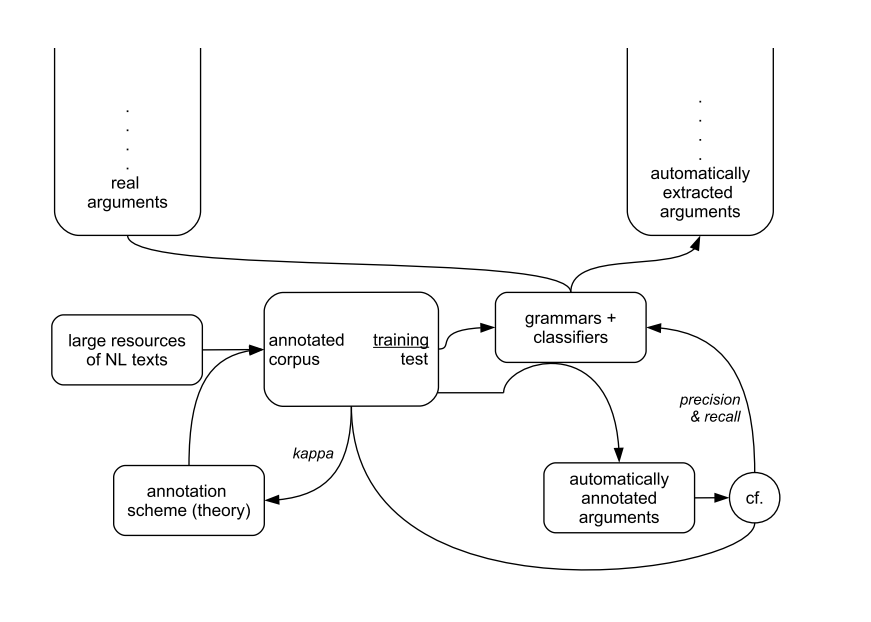
\includegraphics[scale=0.45]{images/NLP_techniques.png}
	\end{center}
	\caption{
		Natural language processing techniques
		\\
		\textbf{Source:} \cite{Budzynska2015}
	}
	\label{NLP_techniques}
\end{figure}

In general, argument mining procedure is separated into linguistic and computational part, as described in figure \ref{NLP_techniques}. Regarding the linguistic part, large corpora of manually annotated argument data are being created based on a common agreement among annotators about argument's structure. On the other hand, the computational part is separated into two main styles of automation, the structural and the statistical approach. (\cite{Budzynska2015}) \par

In \textbf{structural or grammar approach}, linguists aim to retrieve lexical patterns, rules or categories while annotating a training corpus. For example, it might be noticed that words like "because", "since", "however" are signs of arguments inside a specific corpus (\cite{Budzynska2015}). These signs are called indicators, and point out the connection between claims and premises inside a text (\cite{Lawrence2015}). Indicators are declared as linguistic expressions that connect statements and provide an unambiguous recognition of argumentative structure (\cite{Webber2012}). \par

A lot of research has been applied in order to be found words and expressions revealing argumentative structure (\cite{van2007argumentative}, \cite{knott1994using}). Apart from indicators, other structural techniques have been applied for argument mining. Such techniques are argumentation schemes (\cite{Feng2011}), dialogical context (\cite{Budzynska2014}), and semantic context (\cite{Cabrio2012}) or a combination of them. \par

In \textbf{statistical approach}, linguists are replaced by algorithms. These algorithms are basically classifiers developed for automating the argument annotation procedure (\cite{Budzynska2015}). The first attempts for the before mentioned automation were made in (\cite{Moens2007}), in which text is separated into sentences, and then each sentence is classified as argumentative or non-argumentative based on its lexical or syntactic features. As a result, (\cite{Palau2009}) presented an additional separation of argumentative sentences as premises or conclusions. As regards the automatic recognition of argumentative schemes, it was introduced in (\cite{Walton2011}) and it was based on the idea of connecting each scheme with a group of indicators. The paper's proposal is first indicating the arguments included in text, and then matching them to a given list of argument schemes. (\cite{Feng2011}) classifies annotated argumentation structures into a list of five common argumentation schemes. In (\cite{Lippi2015}), the authors describe a framework for claim detection in unstructured data-sets without any contextual information. Because arguments are often expressed through rhetorical structures, the previously mentioned framework was built based on an SVM classifier which captures similarities among parse trees via Tree Kernels. This method is used for measuring likeliness of two trees regarding their common substructures. Furthermore, Habernal and Gurevych (\cite{Habernalt2016}) try to evaluate argument convincingness by assessing their qualitative properties. Using an annotated corpus of 26,000 sentences, their purpose is to predict which argument is more convincing between a pair of arguments and to rank arguments regarding the topic and their convincingness, through the usage of SVM and LSTM algorithms. \par

Various traditional machine learning algorithms have been employed in the context of argument mining (Figure \ref{Machine_learning_algorithms}). More specifically, most of the  algorithms that have been implemented are Support Vector Machines (\cite{Mochales2011}; \cite{Park2015}; \cite{Stab2014}; \cite{Eckle-Kohler2015}), Logistic Regression (\cite{Levy2014}; \cite{Rinott2015}), Naive Bayes classifiers (\cite{Mochales2011}; \cite{Biran2011}; \cite{Park2015}; \cite{Eckle-Kohler2015}), Maximum Entropy classifiers (\cite{Mochales2011}), and Decision Trees and Random Forests (\cite{Stab2014}; \cite{Eckle-Kohler2015}). All mentioned classifiers are trained in labeled corpora. Thus, some parts of the annotated text are given, alongside with the associated label, and during training stage a model is being produced. This model is used to perform predictions on new unlabeled text. (\cite{Lippi2016}) \par

\begin{figure}[!h]
	\begin{center}
		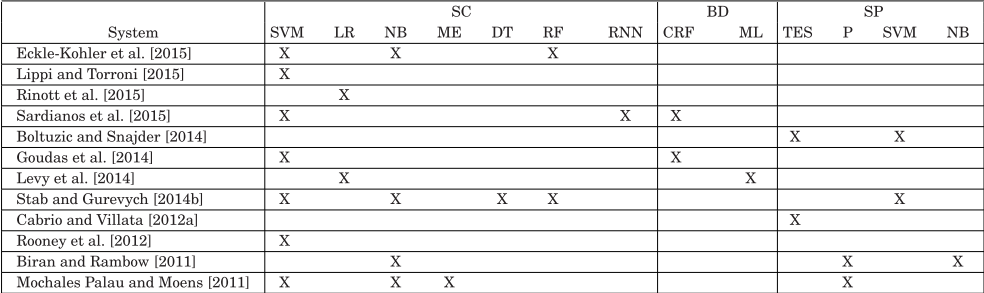
\includegraphics[scale=0.4]{images/Statistical-techniques_used.png}
	\end{center}
	\caption{
		Machine learning algorithms that have been used for argument mining
		\\
		\textbf{Source:} \cite{Lippi2016}
	}
	\label{Machine_learning_algorithms}
\end{figure}

Despite the fact that researchers have tried to make a comparison between these algorithms, there is no clear proof of which classifier is more appropriate for argumentation mining. In fact, most of the research efforts have been settled down on finding appropriate features for improving performance instead of implementing new specifically designed models and algorithms for solving argument identification problem (\cite{Lippi2016}). \par

To sum up, a number of different approaches have been applied to argument identification problem. The research community solutions are ranging from linguistic techniques (\cite{GarciaVillalba2012}) and topic modeling (\cite{Lawrence2014}), to supervised machine learning algorithms( firstly implemented by \cite{Moens2007}). \par

